% David Koch

\documentclass[
	headings=optiontotocandhead,% Erweiterung für das optionale Argument der
	% Gliederungsbefehle aktiviert.
	oneside,
	numbers=noenddot,% Keine Punkte am Ende der Gliederungsnummern und davon
	% abgeleiteten Nummern
	toc=flat, %Flache TOC --- kann man anpassen (auskommentieren)
	10pt, % Schriftgröße
	parskip=full, % Abstand zwischen Absätzen (ganze Zeile)
	listof=totoc, % Verzeichnisse im Inhaltsverzeichnis aufführen
	listof=flat, % mehr Abstand für grosse Zahlen
	numbers=noenddot, % kein Punkt am Ende bei Nummern
	%%enlargefirstpage,% Gibt es bei scrartcl nicht!!!!
	bibliography=totoc, % Literaturverzeichnis im Inhaltsverzeichnis aufführen
	%index=totoc, % Index im Inhaltsverzeichnis aufführen
	%captions=tableheading, % Beschriftung von Tabellen für Ausgabe oberhalb
	% der Tabelle formatieren
	%draft % Status des Dokuments (final/draft) draft hinzufügen zum anziegen
	%%der zeilen ende
	a4paper,DIV=14,
	% captions=tablesignature,
]{scrartcl}

\setcounter{secnumdepth}{3}

\usepackage[T1]{fontenc}
\usepackage[utf8]{inputenc}

\usepackage[english, ngerman]{babel, varioref} % your native language must be the last one!!

\usepackage{lastpage}
\usepackage{listings}
\usepackage{blindtext}

%% Aufzählungen nicht so weit einrücken
\usepackage[inline]{enumitem}
%\setitemize{leftmargin=*}
% Listen etwas wenige einrücken, erfordert enumitem
\setitemize{labelindent=2em,labelsep=0.5cm,leftmargin=12ex}

\usepackage{lmodern}

\usepackage{xspace}

\usepackage{graphicx}
\graphicspath{ {../../assets} {../../assets/Planung/Risikoanalyse} }

%%? \usepackage{textcomp}
\usepackage[hyphens]{url}
\usepackage{makeidx}
\makeindex
%%? \usepackage{graphicx}
\usepackage[numbers]{natbib}
\PassOptionsToPackage{normalem}{ulem}
\usepackage{ulem}

\usepackage{needspace}

\setlength\partopsep{0.5ex}%schoenere Listen
\usepackage[bottom]{footmisc}%fussnote ganz unten

\usepackage[]{microtype}
\UseMicrotypeSet[protrusion]{basicmath} % disable protrusion for tt fonts

\usepackage{multirow}   % Allows table elements to span several rows.
\usepackage{booktabs}   % Improves the typesettings of tables.
\usepackage{subcaption} % Allows the use of subfigures and enables their referencing.
\usepackage[ruled,linesnumbered]{algorithm2e} % Enables the writing of pseudo code.
\usepackage[usenames,dvipsnames,table]{xcolor} % Allows the definition and use of colors. This package has to be included before tikz.
\usepackage{nag}       % Issues warnings when best practices in writing LaTeX documents are violated.
\usepackage{todonotes} % Provides tooltip-like todo notes.
\usepackage{pdflscape}

\usepackage{color}
\usepackage[binary-units]{siunitx}

%% Override default figure placement To be within the flow of the text rather
%% than on it's own page.
% \usepackage{float}
% \makeatletter
% \def\fps@figure{H}
% \makeatother

%% bei vielen Bildern o.ä sinnvoll: Seite muss nicht bis ganz unten gefüllt werden
% \raggedbottom

%\usepackage{footbib} %  footcite, needs other tooling
%% for pandoc2 images
\makeatletter
\def\maxwidth{\ifdim\Gin@nat@width>\linewidth\linewidth\else\Gin@nat@width\fi}
\def\maxheight{\ifdim\Gin@nat@height>\textheight\textheight\else\Gin@nat@height\fi}
\makeatother
% Scale images if necessary, so that they will not overflow the page
% margins by default, and it is still possible to overwrite the defaults
% using explicit options in \includegraphics[width, height, ...]{}
\setkeys{Gin}{width=\maxwidth,height=\maxheight,keepaspectratio}

%% bessere Suche im PDF
\input{glyphtounicode}
\pdfgentounicode=1
%%%%%%%%%%%%%%%%%%%%%%%%%%%%%%%%%%%%%%%%%%%%%%%%%%%%%%%%%%%%%%%%%%%%%%%%%%%%%%%%%%

%  Kopf und Fußzeilen -- links und rechts verschieden
\newcommand{\kopfbild}{\voffset7mm
\includegraphics[width=25mm]{HTL3RLogo}}
\newcommand{\kopfHTL}{\sffamily{\textbf{\large{Projekthandbuch HTL3R}}}}

\usepackage[automark,footsepline,plainfootsepline]{scrlayer-scrpage}
\setkomafont{pageheadfoot}{\normalcolor\footnotesize\scshape}
\setkomafont{pagenumber}{\normalfont\normalsize}
\clearpairofpagestyles
\ihead{\headmark}
\ihead{\kopfbild}
\ohead{\kopfHTL}
\ifoot{\smaller{Höhere Technische Bundeslehranstalt Wien 3 | Rennweg 89b | 1030 Wien | \textcolor{orange}{www.htl.rennweg.at}}}
\ofoot{Seite \pagemark/\pageref{LastPage}}
\ModifyLayer[addvoffset=-.6ex]{scrheadings.foot.above.line}% Linie verschieben
\ModifyLayer[addvoffset=-.6ex]{plain.scrheadings.foot.above.line}% Linie verschieben
\setlength{\headheight}{32pt}

% alle Seiten mit Kopfzeile
%\renewcommand{\chapterpagestyle}{scrheadings}

%% Code Beispiele
%% eine Variante
\usepackage{listings}
\renewcommand{\lstlistingname}{\inputencoding{utf8}Listing}

\usepackage{tabularx}
\usepackage{scrhack}

\usepackage{array}
\newcommand\Tstrut{\rule{0pt}{3.2ex}}         % = `top' strut
\newcommand\Bstrut{\rule[-1.5ex]{0pt}{0pt}}   % = `bottom' strut

\newenvironment{nstabbing}
	{\setlength{\topsep}{-\parskip}
		\setlength{\partopsep}{-\parskip}
		\tabbing}
	{\endtabbing}

\usepackage{titlesec}
% \titleformat{?Überschriftenklasse?}[Absatzformatierung?]{?Textformatierung?} {?Nummerierung?}{?Abstand zwischen Nummerierung und Überschriftentext?}{?Code vor der Überschrift?}[?Code nach der Überschrift?]
\titleformat{\section}[hang]{\Large\bfseries\sffamily}{\thesection\quad}{-1.2ex}{}
\titleformat{\subsection}[hang]{\large\bfseries\sffamily}{\thesubsection\quad}{-1.2ex}{}
\titleformat{\subsubsection}[hang]{\large\bfseries\sffamily}{\thesubsubsection\quad}{-1.2ex}{}
\titleformat{\paragraph}[hang]{\large\bfseries\sffamily}{\theparagraph\quad}{-1.2ex}{}

% \titlespacing{?Überschriftenklasse?}{?Linker Einzug?}{?Platz oberhalb?}{?Platz unterhalb?}[?rechter Einzug?]
\titlespacing{\section}{0pt}{6pt}{6pt}
\titlespacing{\subsection}{0pt}{6pt}{0pt}
\titlespacing{\subsubsection}{0pt}{6pt}{0pt}
\titlespacing{\paragraph}{0pt}{6pt}{0pt}

%% sollte das letzte Package sein
\usepackage[unicode=true,
bookmarks=true,bookmarksnumbered=false,bookmarksopen=false,
breaklinks=true,pdfborder={0 0 0},backref=false,colorlinks=false]
{hyperref}
\hypersetup{pdftitle={Fenrir Risikoanalyse},
	pdfauthor={David Koch},
	pdfsubject={DA},
	pdfkeywords={5CN, Fenrir, DA}}
\urlstyle{same} % don't use monospace font for urls

% Auch Fußnoten bündig ausrichten
\deffootnote[]{1em}{1em}{\textsuperscript{\thefootnotemark\ }}
%% setup
\sloppy % weniger Meldungen
\voffset7mm % etwas nach unten

%%%%%%%%%%%%%%%%%%%%%%%%%%%%%%%%%%%%%%%%%%%%%%%%%%%%%%%%%%%%%%%%%%%%%%%%%%%%%%%%%%
\begin{document}
%% schöner: 10000 -- gar keine, 1000 als Mittelweg
\clubpenalty = 10000 % Schusterjungen verhindern
\widowpenalty = 10000 % Hurenkinder verhindern
\displaywidowpenalty = 10000

{\sffamily{\textbf{\LARGE{\textcolor{orange}{Spielregeln}}}}}\\
\noindent\rule{\textwidth}{0.1pt}
\begin{nstabbing}
	\hspace{4cm}\=\hspace{4cm}\=\hspace{4cm}\=\kill
	Projekttitel: \> \textbf{Fenrir}\\
	Auftraggeber: \> \textbf{Christian Schöndorfer}\\
	Auftragnehmer: \> \textbf{David Koch}\\
	Schuljahr: \> \textbf{2024/25}
	\> Klasse: \> \textbf{5CN}\\
\end{nstabbing}
{\smaller
	\begin{tabularx}{\textwidth}{l l l l}
	\hline
	\textbf{Version} & \textbf{Datum} & \textbf{Autorin/Autor} & \textbf{Änderung}\Tstrut  \\
	v1.0 & 13.06.2024 & David Koch & Erstellung der Risikoanalyse (Draft) \\
	v1.1 & 16.06.2024 & David Koch & Ergänzung der Risikomaßnahmen\Bstrut \\
	\hline
	\end{tabularx}
}

\section{Projektrisikoanalyse}
Risiken sind Ereignisse, die einen realen Schaden anrichten. Der Schaden kann sich im Projektmanagement auf einen oder mehrere der Faktoren Zeit, Kosten, Qualität und Nutzen des Produktes auswirken. Ziel ist es, bereits im Projektvorfeld Maßnahmen zur Risikovermeidung zu treffen oder für den Eintrittsfall einen Plan B (Maßnahmen) parat zu haben.

\subsection{Identifikation der Risiken}
Die Risiken sollen systematisch durch Betrachtung der untenstehenden Risikoquellen identifiziert und dokumentiert werden. (Für die Struktur siehe \autoref{sec:risikotabelle})

\begin{enumerate}
	\item{Die Funktionalitäten/Anforderungen hinsichtlich Risiken analysieren, die Risiken identifizieren und zu der Liste hinzufügen.}
	\item{Welche Risiken können aus den angrenzenden Gebieten, wie z.B. Server und Infrastruktur eintreten?}
	\item{Brainstorming im Team mit Einbeziehung von Experten, um weitere Risiken zu identifizieren [Beispiele: Planungsfehler, Knowhow-Defizite des Teams, Umfeldveränderungen]. Diese können bereits bei der Stakeholderanalyse identifiziert worden sein.}
	\item{
		Checkliste mit den bekanntesten branchenüblichen Risiken kontrollieren und zutreffende Risiken in die Liste aufnehmen
		\begin{itemize}
			\item Definition der Aufgabenstellung (zu grob)
			\item Analyse der Machbarkeit
			\item verfügbare Erfahrung (neue Technologien, Tools, Methoden)
			\item keine Einbindung der End-User/weiterer Stakeholder
			\item "'Vergoldung"' (Entwickler neigen dazu, mehr Leistungen zu planen als vereinbart sind)
			\item Unklare Verantwortlichkeiten
			\item Unzureichendes oder nicht kontinuierliches Risiko-Management
		\end{itemize}
		}
\end{enumerate}

\subsection{Bewertung der Risiken}
Die einzelnen Risiken sollen jeweils durch die \textbf{Eintrittswahrscheinlichkeit (P)} und das \textbf{Schadensausmaß bei Eintritt (A)} bewertet werden. Der \textbf{Risikofaktor (RF)} berechnet sich dann aus der Multiplikation dieser zwei Werte: RF = P x A\\
Wichtig ist, dass nach der Bewertung die Risiken nach absteigendem Risikofaktor (RF) sortiert werden, so dass die Risiken mit höchster Wertigkeit ganz oben in der Liste stehen.

\begin{landscape}
\subsection{Risikotabelle}
	\begin{table}[h]
		\begin{tabularx} {.7925\paperheight} {
				|>{\hsize=.02\paperheight}X
				|>{\hsize=.1\paperheight}X
				|>{\hsize=.16\paperheight}X
				|>{\hsize=.02\paperheight}X
				|>{\hsize=.02\paperheight}X
				|>{\hsize=.03\paperheight}X
				|>{\hsize=.08\paperheight}X
				|>{\hsize=.18\paperheight}X
				|>{\hsize=.05\paperheight}X|
			}
			
			\hline
			\rowcolor[HTML]{D9D9D9} 
			\rule{0pt}{17pt}
			\textbf{\normalsize{\#}} & \textbf{\normalsize{Bezeichnung}} & \textbf{\normalsize{Beschreibung}} & \textbf{\normalsize{P}} & \textbf{\normalsize{A}} & \textbf{\normalsize{RF}} & \textbf{\normalsize{Verzögerung (in Wochen)}} & \textbf{\normalsize{Maßnahme(n) zur Reduktion}} & \textbf{\normalsize{Kosten}} \\ \hline
			1 & Ungeplanter Ausfall eines PM & Ein Projektmitarbeiter fällt aufgrund eines unvorhersehbaren Vorfalls (z.B. Unfall) für eine längere Dauer aus. & 30 & 60 & 1800 & >=1 & Jedem Ziel ein zweites Teammitglied mit gleichem oder ähnlichem Kompetenzbereich zuweisen um beim Ausfall keine Zeit zu verlieren & 0€\\ \hline
			2 & Termin nicht im Projektterminkalender eingetragen & Ein Termin, wie z.B. ein Urlaub eines PM oder ein Statusmeeting mit den Betreuern, wurde nicht in den Projektterminkalender eingetragen. Somit kann es dazu kommen, dass ein PM auf diesen Termin vergisst. & 20 & 30 & 600 & >=0 & In der Vorprojektphase bereits alle Teammitglieder auffordern ihren Urlaub in den Projektterminkalender unter MS Teams einzutragen, bei Meetings so früh es geht eintragen (sobald sie ausgemacht worden sind) & >=0€\\ \hline
			3 & Unerreichbarkeit eines Betreuers & Mindestens einer der Projektbetreuer ist für eine Dauer nicht erreichbar. Somit kann das Projektteam z.B. nicht wichtige Rückfragen bezüglich der Projektumsetzung oder des Projektablaufs stellen. & 50 & 40 & 2000 & >=0 & Private Mobiltelefonnummern der Projektbetreuer abfragen, um diese im Fall der Fälle für eine direkte Kontaktaufnahme zu nutzen & 0€\\ \hline
			4 & Wasserbehälter undicht & Eine OT-Komponente, die Wasser enthält oder durch sich durchfließen hat (Rohr, Pumpe, Tank, …) ist undicht geworden und kann unter Umständen einen Wasserschaden anrichten → Siehe Risiko \#5 & 75 & 10 & 750 & >=0 & Beim Aufbau der OT-Betriebszellen alles so gut es abdichten, bei neuen Beschädigungen an der Abdichtung stets Tücher zur Eingrenzung der ausgelaufenen Flüssigkeit mit den OT-Betriebszellen mitführen & 0€\\ \hline
			5 & Irreversibler Schaden am/im OT-Netzwerk & Es ist ein irreversibler Schaden an einer OT-Komponente entstanden, z.B. Rohrbruch oder Pumpenmotor defekt & 15 & 60 & 900 & >=1 & Schaden reparieren bzw. beschädigtes Bauteil neu bestellen & 10€ bis 200€\\ \hline
		\end{tabularx}
	\end{table}

	\begin{table}[h]
		\begin{tabularx} {.7925\paperheight} {
				|>{\hsize=.02\paperheight}X
				|>{\hsize=.1\paperheight}X
				|>{\hsize=.16\paperheight}X
				|>{\hsize=.02\paperheight}X
				|>{\hsize=.02\paperheight}X
				|>{\hsize=.03\paperheight}X
				|>{\hsize=.08\paperheight}X
				|>{\hsize=.18\paperheight}X
				|>{\hsize=.05\paperheight}X|
			}
			
			\hline
			\rowcolor[HTML]{D9D9D9} 
			\rule{0pt}{17pt}
			\textbf{\normalsize{\#}} & \textbf{\normalsize{Bezeichnung}} & \textbf{\normalsize{Beschreibung}} & \textbf{\normalsize{P}} & \textbf{\normalsize{A}} & \textbf{\normalsize{RF}} & \textbf{\normalsize{Verzögerung (in Wochen)}} & \textbf{\normalsize{Maßnahme(n) zur Reduktion}} & \textbf{\normalsize{Kosten}} \\ \hline
			6 & Fehler bei der Versionierung & Es ist ein Fehler in der Versionierung der Projektdateien (Planungsdokumente, SPS-Programme, …) passiert. (Dazu gehört z.B. auch ein Force-Push auf das Projekt-GitHub-Repository!) & 20 & 5 & 100 & 0 & Alle Projektmitglieder sollen die GitHub-Nomenklatur, die Spielregeln sowie die Regel, dass keine Force-Pushes auf das Repository erlaubt sind, beachten. & 0€\\ \hline
			7 & Veraltete Dokumentation & Ein von einem PM geschriebene Dokumentation wurde nach Änderungen an der Topologie nicht auf den neuesten Stand gebracht, womit mithilfe dieser Doku der derzeitige Topologiezustand nicht mehr replizierbar ist & 30 & 15 & 450 & >0 & Dokumentation nach Abänderung(en) stets von anderen Projektmitarbeitern peer-reviewen lassen & 0€\\ \hline
			8 & Fernzugriff auf UCS fällt aus & Der VPN-Zugriff auf die UCS-Infrastruktur an der HTL Rennweg ist z.B. wegen eines Stromausfalls für eine gewisse Zeitspanne nicht funktionsfähig. & 80 & 80 & 6400 & >0 & Auf dem Home-Server eines Teammitglieds in "'kleinem Maßstab"' die gleiche Umgebung wie auf der UCS-Infrastruktur an der HTL Rennweg erstellen, sodass Provisionierungskonfigurations oder andere Arbeit im IT-Netzwerk ausgelagert werden kann, bis die Schul-UCS wieder läuft & 0€\\ \hline
			9 & Yggdrasil-UCS-Dokumentation unzureichend & Die Dokumentation der UCS und dessen Provisionierung/Konfiguration ist im Diplomarbeitsbuch der Diplomarbeit Yggdrasil unzureichend/fehlerhaft. & 100 & 30 & 3000 & 0 & Laut den Projektbetreuern ist dieses Risiko bereits eingetreten (weil das Yggdrasil-Diplomarbeitsbuch bereits fertig ist und so nicht mehr verändert werden kann), daher ist eine Gegenmaßnahme nicht sinnvoll bzw. unmöglich & 0€\\ \hline
			10 & OT-Betriebszelle geht verloren & Eine gesamte OT-Betriebszelle inklusive Aktorik/Sensorik sowie die SPS und dessen Verkabelung ist verloren gegangen. & 5 & 90 & 450 & 3 & Beim Transport sowie bei der Lagerung der OT-Betriebszellen achtsam sein, dass alles korrekt abgeschlossen/verriegelt ist, so, dass sie nicht geklaut werden kann. & 300€ bis 500€\\ \hline
		\end{tabularx}
	\end{table}

	\begin{table}[h]
		\begin{tabularx} {.7925\paperheight} {
				|>{\hsize=.02\paperheight}X
				|>{\hsize=.1\paperheight}X
				|>{\hsize=.16\paperheight}X
				|>{\hsize=.02\paperheight}X
				|>{\hsize=.02\paperheight}X
				|>{\hsize=.03\paperheight}X
				|>{\hsize=.08\paperheight}X
				|>{\hsize=.18\paperheight}X
				|>{\hsize=.05\paperheight}X|
			}
			
			\hline
			\rowcolor[HTML]{D9D9D9} 
			\rule{0pt}{17pt}
			\textbf{\normalsize{\#}} & \textbf{\normalsize{Bezeichnung}} & \textbf{\normalsize{Beschreibung}} & \textbf{\normalsize{P}} & \textbf{\normalsize{A}} & \textbf{\normalsize{RF}} & \textbf{\normalsize{Verzögerung (in Wochen)}} & \textbf{\normalsize{Maßnahme(n) zur Reduktion}} & \textbf{\normalsize{Kosten}} \\ \hline
			11 & Physischer Zugang zum OT-Netzwerk nicht möglich & Der physische Zugang zum OT-Netzwerk ist nicht mehr möglich aufgrund von z.B. Urlaub eines PMs, bei dem derzeit das OT-Netzwerk aufgebaut ist. & 100 & 80 & 8000 & >=1 & Auf die Urlaubszeit der Person, die derzeit das OT-Netzwerk bei sich zuhause lagert, bezogen: Urlaubszeit früh planen und mit dem restlichen Team absprechen sowie in den Projektterminkalender eintragen (siehe Risiko \#2) & 0€\\ \hline
			12 & Missverständnis in der Kommunikation nach innen/außen & Bei der Kommunikation z.B. innerhalb eines Meetings mit einem Betreuer, Sponsor oder nur einem Teammitglied ist ein Missverständnis entstanden, welches sich negativ auf die Umsetzung des Projektes auswirken kann & 90 & 20 & 1800 & >=0 & ... & >=0€\\ \hline
			13 & Fehleinschätzung der Dauer der Umsetzungsphase & Die während der Planungsphase des Projektes getroffene Einschätzung der Arbeitsdauer der Umsetzungsphase ist zu lässig. & 60 & 30 & 1800 & >=1 & ... & 0€\\ \hline
			14 & Grober Inhaltsfehler in der Dokumentation & Bei der Dokumentation eines Arbeitsbereiches ist ein grober Fehler unterlaufen, wodurch die Dokumentation nicht mehr Realität abbildet und somit (zum Teil) unbrauchbar wird. & 10 & 35 & 350 & >0 & Dokumentationen stets am besten von allen Teammitgliedern peer-reviewen lassen, sodass beim Auftreten solcher groben Inhaltsfehler diese so früh wie möglich ausgebessert werden können & 0€\\ \hline
			15 & Firewall-VDOMs nicht umsetzbar wie geplant & Die Für die Projekttopologie nötige Aufteilung von physischen FortiGate 60F-FWs in mehrere virtuelle FWs kann nicht wie geplant verlaufen (wegen Konfigurationsschwierigkeiten z.B.). & 25 & 40 & 1000 & >1 & Teure Maßnahme: Mehr Hardware-FWs beantragen; Billige Maßnahme(n): Auf pfSense-FWs umsteigen oder Topologie kleiner gestalten, sodass nicht so viele Firewalls gebraucht werden & >=0€\\ \hline
			16 & Rechtliche Grundlagen der Website unzureichend & Das Impressum (Kontaktdaten) auf der Website www.fenrir-ot.at ist für die rechtlichen Grundlagen Österreichs bzw. der EU unzureichend & 20 & 70 & 1400 & >0 & Mit vorherigen Diplomarbeitsteam sprechen und sich von ihren Webseiten inspirieren lassen sowie mit z.B. Herrn Prof. Oppeker über die Impressumspflichten reden & 0€\\ \hline
		\end{tabularx}
	\end{table}
	
	\begin{table}[h]
		\begin{tabularx} {.7925\paperheight} {
				|>{\hsize=.02\paperheight}X
				|>{\hsize=.1\paperheight}X
				|>{\hsize=.16\paperheight}X
				|>{\hsize=.02\paperheight}X
				|>{\hsize=.02\paperheight}X
				|>{\hsize=.03\paperheight}X
				|>{\hsize=.08\paperheight}X
				|>{\hsize=.18\paperheight}X
				|>{\hsize=.05\paperheight}X|
			}
			
			\hline
			\rowcolor[HTML]{D9D9D9} 
			\rule{0pt}{17pt}
			\textbf{\normalsize{\#}} & \textbf{\normalsize{Bezeichnung}} & \textbf{\normalsize{Beschreibung}} & \textbf{\normalsize{P}} & \textbf{\normalsize{A}} & \textbf{\normalsize{RF}} & \textbf{\normalsize{Verzögerung (in Wochen)}} & \textbf{\normalsize{Maßnahme(n) zur Reduktion}} & \textbf{\normalsize{Kosten}} \\ \hline
			17 & Abschweifung von der geplanten AD-Struktur & Die in der Planungsphase definierte AD-Struktur kann nicht exakt eingehalten werden (aufgrund von einer zu umständlichen Umsetzung für den Nutzen/Zweck). & 60 & 5 & 300 & 0 & AD-Struktur auf eine Struktur die passt umgestalten, d.h. Change-Request nötig, ist aber nichts dramatisches. & 0€\\ \hline
			18 & Angriffsszenario führt zu ungeplantem Schaden & Ein geplanter Angriff auf die Projekttopologie (als Teil eines Zieles der Diplomarbeit) führt zu ungeplanten Schäden, z.B. siehe Risiko \#5 & 10 & 50 & 500 & >0 & Angriffe klein halten und vorsichtig durchplanen, sodass kein ungeplanter Schaden überhaupt entstehen kann. & >=0€\\ \hline
			19 & Zielerfüllungstermin nicht eingehalten & Der in der Zieldefinition eines Zieles niedergeschriebene Liefertermin kann nicht eingehalten werden (Verspätung). & 50 & 60 & 3000 & >0 & Die in den nächsten 30 Tagen anstehenden Zielerfüllungstermine stets im Auge behalten und in allen Statusmeetings mit oder ohne die Betreuern besprechen, ob diese bereits erfüllt worden sind oder wie der derzeitige Erfüllungsstatus ist. & 0€\\ \hline
			20 & Meilensteintermin nicht eingehalten & Der in der Meilensteindefinition eines Meilensteins niedergeschriebene Abschlusstermin kann nicht eingehalten werden (Verspätung). & 20 & 60 & 1200 & >0 & Die in den nächsten 30 Tagen anstehenden Meilensteintermine stets im Auge behalten und in allen Statusmeetings mit oder ohne die Betreuer besprechen, ob alle Ziele für diesen Meilenstein bereits erfüllt worden sind oder wie der derzeitige Erfüllungsstatus ist. & 0€\\ \hline
		\end{tabularx}
	\end{table}
	
	\begin{table}[h]
		\begin{tabularx} {.7925\paperheight} {
				|>{\hsize=.02\paperheight}X
				|>{\hsize=.1\paperheight}X
				|>{\hsize=.16\paperheight}X
				|>{\hsize=.02\paperheight}X
				|>{\hsize=.02\paperheight}X
				|>{\hsize=.03\paperheight}X
				|>{\hsize=.08\paperheight}X
				|>{\hsize=.18\paperheight}X
				|>{\hsize=.05\paperheight}X|
			}
			
			\hline
			\rowcolor[HTML]{D9D9D9} 
			\rule{0pt}{17pt}
			\textbf{\normalsize{\#}} & \textbf{\normalsize{Bezeichnung}} & \textbf{\normalsize{Beschreibung}} & \textbf{\normalsize{P}} & \textbf{\normalsize{A}} & \textbf{\normalsize{RF}} & \textbf{\normalsize{Verzögerung (in Wochen)}} & \textbf{\normalsize{Maßnahme(n) zur Reduktion}} & \textbf{\normalsize{Kosten}} \\ \hline
			21 & Prototyp für Betreuer/Sponsor unzureichend & Ein Prototypmodell einer OT-Betriebszelle oder auch Teile des IT-Netzwerks sind für einen Betreuer/Sponsoren unzureichend in dem Sinne, dass es nicht den von ihnen gestellten Erwartungen entspricht. & 15 & 50 & 750 & >0 & Bereits bei der Entwicklung des Prototypmodells Absprache mit den Betreuern/Sponsoren halten, wie die Vorstellungen sind. & >0€\\ \hline
			22 & Probleme bei der Lizenzierung der FWs/Guardian & Die Lizenzen für die FortiGate-FWs oder für die Nozomi Guardian sind grundlegend ungültig, nicht für den gesamten Umsetzungszeitraum über gültig oder geben nicht die für die geplante Projektumsetzung benötigte Ressourcen frei. & 20 & 70 & 1400 & >=1 & Mit dem Auftraggeber bzw. Sponsor vorzeitig alle benötigten Lizenzen abklären und bestenfalls vor dem Beginn der Umsetzungsphase diese erhalten. & >=0€\\ \hline
			23 & Fehlverkabelung der Aktorik/Sensorik & Bei der Verkabelung der Aktorik sowie Sensorik untereinander und/oder mit der SPS ist ein Flüchtigkeitsfehler unterlaufen. & 60 & 10 & 600 & >=0 & Vor der tatsächlichen Verkabelung einen Schaltplan machen, nicht alles auf einmal verkabeln und Stück für Stück alles vorsichtig richtig machen, Peer-Reviewing durch Teammitglieder auch möglich & 0€\\ \hline
			24 & Fehlprogrammierung einer SPS & Bei der Programmierung einer SPS unterläuft ein Fehler, welcher bei der Steuerung der Aktorik/Sensorik zu unbeabsichtigtem Verhalten führt. & 60 & 10 & 600 & >=0 & SPS-Programme von anderem Teammitgliedern peer-reviewen lassen und falls möglich zuerst simulieren bevor diese auf echter Hardware laufen. & 0€\\ \hline
			25 & Fehlkonfiguration einer FortiGate-FW & Bei der Konfiguration einer FortiGate-FW unterläuft ein Fehler, welcher zu Problemen (zu viel erlaubt bzw. geblockt z.B.) bei dem Datenverkehr im Netzwerk führt. & 40 & 10 & 400 & >=0 & FW-Konfigurationen ausführlich kommentieren und von anderen Team-Mitgliedern peer-reviewen lassen & 0€\\ \hline
			26 & Transportschaden & Beim Transport einer OT-Betriebszelle ist in dieser ein irreversibler Schaden entstanden (z.B. Holz gebrochen). & 25 & 40 & 1000 & >=1 & Beim Transport einer OT-Betriebszelle diese stets sicher handhaben. & >10€\\ \hline
		\end{tabularx}
	\end{table}
\end{landscape}

\subsection{Risikoportfolio}
Die Risiken werden jetzt aus der Tabelle in das Portfolio übertragen und A/B/C-Risiken identifiziert. Für A/B-Risiken müssen ganz konkrete Gegenmaßnahmen geplant werden — einerseits um die Eintrittswahrscheinlichkeit zu verringern, andererseits um das Schadensausmaß zu verringern. A-Risiken müssen unbedingt sofort mit dem Auftraggeber besprochen werden!
\begin{figure}[h]
	\centering
	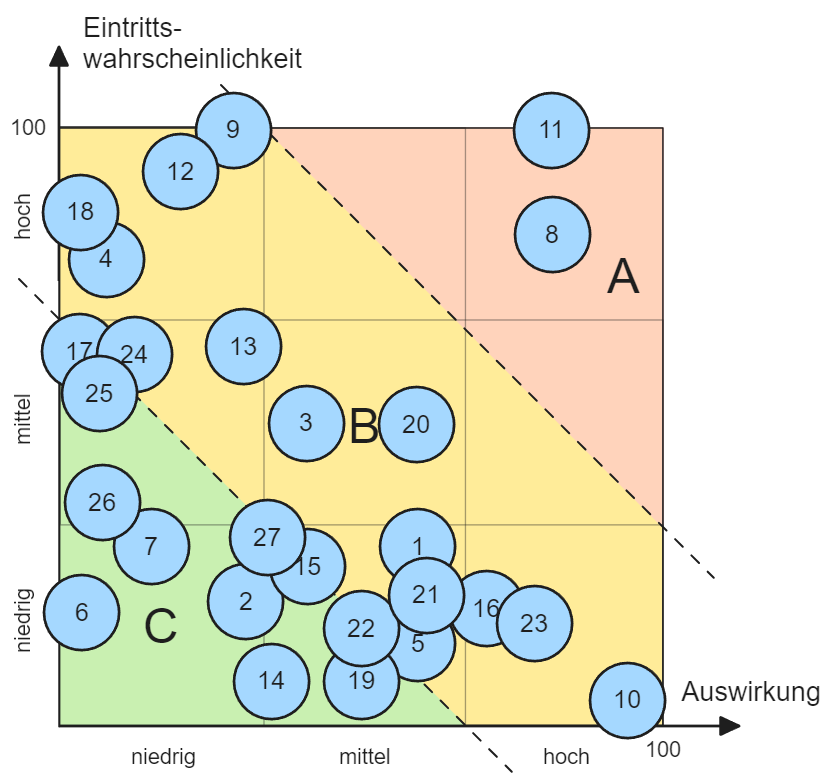
\includegraphics[width=1\linewidth]{risikoportfolio}
	\caption[]{Visualisierung der Risikotabelle (Risikoportfolio)}
\end{figure}

\end{document}